\documentclass[]{standalone}
\usepackage[utf8]{inputenc}
\usepackage[american]{circuitikz}
\usetikzlibrary{arrows,shapes,calc,positioning}

\usepackage{graphicx}

\newcommand{\myscope}[2] % #1 = name , #2 = rotation angle
{\draw[thick,rotate=#2] (#1) circle (12pt)
 (#1) ++(-0.35,-0.1) -- ++(0.3,0.3) --++(0,-0.3)-- ++(0.3,0.3) --++(0,-0.3);
}

\begin{document}

\pgfmathsetmacro\circuitheight{8}
\pgfmathsetmacro\circuitwidth{18}

\begin{circuitikz}[scale=1]
  % Power rails
  \draw (-1, \circuitheight) to[V, label=24V] (-1, 0); 
  \draw[red, thick] (-1,\circuitheight) to [short, -o] ++(\circuitwidth, 0); 
  \draw[blue, thick] (-1,0) to [short, -o] ++(\circuitwidth, 0); 

    \begin{scope}[xshift=6cm, yshift=4cm]
    \node[draw, minimum width=2cm, minimum height=4cm] (valve) at (0,0) {PID};
    \node[coordinate, ] (vplus) at (-1.4, 1.6) {}; 
    \draw (valve.west |- vplus)  to [short, -*, color=red] (vplus);
    \node[coordinate, ] (vmin) at (-1.4, -1.6) {}; 
    \draw (valve.west |- vmin)  to [short, -*, color=blue] (vmin);
    \node[coordinate, ] (uneg) at (.4, -0.2) {}; 
    \draw (valve.east |- uneg)  to [short, -o] (uneg);
    \node[coordinate, ] (uplus) at (2, 0.2) {}; 
    \draw (valve.east |- uplus)  to [short, -*] (uplus);

    \node[coordinate, ] (refneg) at (-1.4, 0.4) {}; 
    \draw[black!30] (valve.west |- refneg)  to [short, -o] (refneg);
    \node[coordinate, ] (refplus) at (-2.4, 0.8) {}; 
    \draw (valve.west |- refplus)  node[right] {ref} to [short, -*] (refplus);

    \node[coordinate, ] (yneg) at (-1.4, -0.8) {}; 
    \draw[black!30] (valve.west |- yneg)  to [short, -o] (yneg);
    \node[coordinate, ] (yplus) at (-2, -0.4) {}; 
    \draw (valve.west |- yplus)  node[right] {y} to [short, -*] (yplus);
  \end{scope}
  \draw[blue] (vmin) to[short] (vmin |- 0,0);
  \draw[red] (vplus) to[short] (vplus |- 0,\circuitheight);
  \draw[blue] (vmin) to (yneg);
  \draw[blue] (vmin) to (refneg);

  \begin{scope}[xshift=10cm, yshift=4cm]
    \node[draw, minimum width=2cm, minimum height=1.6cm] (valve) at (0,0) {Valve};
    \node[coordinate, ] (vvplus) at (-1.4, 0.6) {}; 
    \draw (valve.west |- vvplus)  to [short, -*, color=red] (vvplus);
    \node[coordinate, ] (vvmin) at (-1.4, -0.6) {}; 
    \draw (valve.west |- vvmin)  to [short, -*, color=blue] (vvmin);
    \node[coordinate, ] (vwhite) at (-1.4, -0.2) {}; 
    \draw (valve.west |- vwhite)  to [short, -o] (vwhite);
    \node[coordinate, ] (vblack) at (-2, 0.2) {}; 
    \draw (valve.west |- vblack)  to [short, -*] (vblack);
  \end{scope}
  \draw[blue] (vvmin) to[short] (vvmin |- 0,0);
  \draw[red] (vvplus) to[short] (vvplus |- 0,\circuitheight);
  \draw[blue] (vwhite) to[short] (vvmin);

  
  \begin{scope}[xshift=14cm, yshift=4cm]
    \node at (0,0) {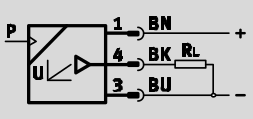
\includegraphics[width=3cm]{pressure-transmitter.png}};
    \node[coordinate] (psplus) at (1.2,.3) {};
    \node[coordinate] (psmin) at (1.2,-.4) {};
    \node[coordinate] (pssignal) at (2,-0.05) {};
    \draw (pssignal) to [short, -*] ++(-1.6,0);
  \end{scope}
  \draw[red] (psplus |- 0,\circuitheight) to [short,-*] (psplus);
  \draw[blue] (psmin |- 0,0) to [short,-*] (psmin);
  %\draw (pssignal |- (0,0) to[sV, color=white, name=S] (pssignal);
  \draw (pssignal) -- ++(0, -3cm) -- ++(-13cm, 0) |- (yplus);
  %\myscope{S}{0}

  %\draw (vplus |- 0,\circuitheight) to [short,] (vplus);
  %\draw (vmin |- 0,0) to [short,] (vmin);
  %\draw (vwhite |- 0,0) to [short,] (vwhite);
  

  \node[spdt, rotate=-90] (sw) at (1.5, 2.5) {};
  \draw (refplus) -| (sw.in);
  \draw (sw.out 1) to[short,] (sw.out 1 |- 0,0);
  \draw (sw.out 2) to[V, a={$u_{i}$},] (sw.out 2 |- 0,0);


  %\node[coordinate, left of=vblack, node distance=3.5cm] (Osc) {};
  %\draw (vblack) to[short] (Osc) to[sV, color=white, name=S2] (Osc |- 0,0);
  %\myscope{S2}{0}
\end{circuitikz}
\end{document}
